\documentclass{standalone}
\usepackage{tikzducks}

\newcommand{\superstripes}{%
	\stripes[color=blue!80!black,width=3,height=1.0,rotate=5] 
	\stripes[color=blue!80!black,width=0.1,rotate=0,distance=0.7,initialx=-1.1,height=2]
}
\pagecolor{gray!20!white}

\begin{document}

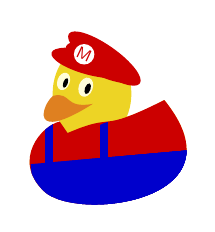
\begin{tikzpicture}
	\duck[
		tshirt=red!80!black,
		peakedcap=red!80!black,
		stripes={\superstripes}
	]
	\fill[white] (0.8,2) circle (0.13);
	\node[red!80!black,rotate=-25] at (0.8,2) {\scalebox{0.6}{\textsf{M}}};
\end{tikzpicture}	

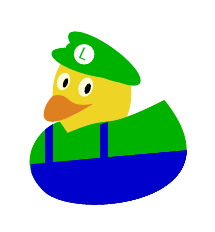
\begin{tikzpicture}
	\duck[
		tshirt=green!70!black,
		peakedcap=green!70!black,
		stripes={\superstripes}
	]
	\fill[white] (0.8,2) circle (0.13);
	\node[green!70!black,rotate=-25] at (0.8,2) {\scalebox{0.6}{\textsf{L}}};
\end{tikzpicture}	
	
\end{document}